\documentclass[11pt,a4paper,reqno]{amsart}

\usepackage[utf8]{inputenc}
\usepackage[T1]{fontenc}
\usepackage{lmodern}
\usepackage{amsmath,amssymb,amsthm,mathtools}
\usepackage{booktabs}
\usepackage{array}
\usepackage{graphicx}
\usepackage{xcolor}
\definecolor{acadblue}{rgb}{0.0, 0.24, 0.52}
\usepackage[margin=2.45cm]{geometry}
\usepackage[colorlinks=true,linkcolor=acadblue,citecolor=acadblue,urlcolor=acadblue]{hyperref}

\newtheorem{theorem}{Theorem}[section]
\newtheorem{proposition}[theorem]{Proposition}
\newtheorem{lemma}[theorem]{Lemma}
\newtheorem{corollary}[theorem]{Corollary}
\theoremstyle{definition}
\newtheorem{definition}[theorem]{Definition}
\theoremstyle{remark}
\newtheorem{remark}[theorem]{Remark}

\numberwithin{equation}{section}
\allowdisplaybreaks

\newcommand{\dd}{\mathrm{d}}
\newcommand{\ii}{\mathrm{i}}
\newcommand{\ee}{\mathrm{e}}
\newcommand{\Rea}{\operatorname{Re}}
\newcommand{\Ima}{\operatorname{Im}}
\newcommand{\Wig}{\mathcal{W}}
\newcommand{\Wtil}{\widetilde{W}}

\title[Wigner Phase-Space and Saddle Coalescence in Riemann's $\Xi$-Function]{Wigner Phase-Space Representation and Complex Saddle-Point Coalescence in the Transverse Wronskian of Riemann's $\Xi$-Function}

\author{Thijs Missiaen}
\address{Independent Researcher, Belgium}
\email{thijs.missiaen@gmail.com}
\urladdr{https://github.com/thijsmissiaen}

\subjclass[2020]{Primary 11M06, 30E15; Secondary 81S30, 42B10, 65D30}
\keywords{Riemann Xi-function, Jacobi theta kernel, transverse Wronskian, Wigner phase-space distribution, Hudson theorem, complex saddle-point coalescence, steepest descent}

\date{October 2026}

\begin{document}

\begin{abstract}
We prove that the inner correlation integral $I(y,t)$ governing the transverse Wronskian $W(d,t) = \frac{1}{2}\partial_d|\Xi(t-\ii d)|^2$ of Riemann's completed $\Xi$-function is proportional to the quantum-mechanical Wigner phase-space distribution $\Wig_\Phi(y,2t)$ of the Jacobi--Riemann kernel $\Phi(u)$, and that its $99.77\%$ real-axis Fourier cancellation at $t=\gamma_1$ is eliminated by shifting the integration contour into the holomorphic strip $|\Ima(x)| < \pi/4$. Our proof combines the holomorphic Jacobi differential identity for $\Phi(-u)=\Phi(u)$, double-exponential decay estimates on the vertical Cauchy walls $\xi = \pm L$, Hermitian reflection symmetry $G_y(-\xi+\ii\eta) = \overline{G_y(\xi+\ii\eta)}$ along horizontal contours, and a pitchfork saddle-point coalescence on the imaginary axis $\xi_* = 0$ for all $|y| \ge y_c(t)$. We further establish that Hudson's theorem and the zero-marginal identity $\int_{\mathbb{R}} I(y,\gamma_k)\,\dd y = 2|\Xi(\gamma_k)|^2 = 0$ force $I(y,\gamma_k)$ to change sign in $y$, while the monotone hyperbolic moment weight $y\sinh(d y)$ amplifies the positive coalesced tail.
\end{abstract}

\maketitle

\section{Introduction}\label{sec:intro}

Let $\xi(s) = \frac{1}{2}s(s-1)\pi^{-s/2}\Gamma(s/2)\zeta(s)$ denote Riemann's completed zeta function, and set $s = \frac{1}{2} + d + \ii t$ with transverse offset $d = \sigma - \frac{1}{2} \in \mathbb{R}$ and spectral height $t \in \mathbb{R}$. Writing $z = -\ii(s - \frac{1}{2}) = t - \ii d$, Riemann's entire function $\Xi(z) := \xi(\frac{1}{2} + \ii z) = R(d,t) + \ii I_{\mathrm{im}}(d,t)$ admits the Fourier--Laplace integral representation \cite{Riemann1859,Polya1926,Titchmarsh1986}
\begin{equation}\label{eq:Xi_integral}
\Xi(t - \ii d) = 2\int_0^\infty \Phi(u)\cosh(d u)\cos(t u)\,\dd u = \int_{-\infty}^\infty \Phi(u)\,\ee^{d u - \ii t u}\,\dd u,
\end{equation}
where the rapidly decaying kernel $\Phi(u)$ is generated by the classic Jacobi theta series $\theta(x) = \sum_{n=-\infty}^\infty \ee^{-\pi n^2 x}$ through
\begin{equation}\label{eq:Phi_def}
\Phi(u) := \sum_{n=1}^\infty \phi_n(u), \qquad \phi_n(u) := \left(2\pi^2 n^4 \ee^{9u} - 3\pi n^2 \ee^{5u}\right)\exp\!\left(-\pi n^2 \ee^{4u}\right).
\end{equation}
By the positivity criteria of Speiser \cite{Speiser1934}, Hinkkanen \cite{Hinkkanen1997}, and Lagarias \cite{Lagarias1999}, the absence of off-critical zeros of $\Xi(t-\ii d)$ in $d > 0$ is intimately linked to the sign of the real part of the logarithmic derivative $\Rea(\xi'(s)/\xi(s)) = W(d,t)/|\Xi(t-\ii d)|^2$, where the \emph{transverse Wronskian} is defined by
\begin{equation}\label{eq:W_def}
W(d,t) := \frac{1}{2}\frac{\partial}{\partial d}\big|\Xi(t-\ii d)\big|^2 = R\,\partial_d R + I_{\mathrm{im}}\,\partial_d I_{\mathrm{im}} = R\,\partial_t I_{\mathrm{im}} - I_{\mathrm{im}}\,\partial_t R.
\end{equation}
When \eqref{eq:W_def} is expanded directly as a double integral over $(u,v) \in \mathbb{R}^2$ along the real axis, numerical and analytical evaluation is obstructed by severe oscillatory cancellation: at the first non-trivial zero $t = \gamma_1 \approx 14.13472514$, positive and negative cosine lobes cancel to $99.7697\%$. The purpose of this article is to resolve this cancellation problem analytically by establishing the exact phase-space and complex-contour structure of $W(d,t)$.

\begin{theorem}[Wigner Phase-Space Identity and Pitchfork Saddle Coalescence]\label{thm:main}
Let $d > 0$ and $t > 0$, and define the mirror coordinates $x = u + v$ and $y = u - v$ with mirror convolution kernel $G_y(x) := \Phi\!\left(\frac{x+y}{2}\right)\Phi\!\left(\frac{x-y}{2}\right)$. Then the following properties hold:
\begin{enumerate}
\item[\textup{(i)}] \textbf{Wigner--Hudson phase-space representation and zero-marginal law:} The transverse Wronskian and its parity-reduced counterpart $\Wtil(d,t) := W(d,t)/d$ admit the exact representations
\begin{equation}\label{eq:W_mirror_thm}
W(d,t) = \frac{1}{2}\int_0^\infty y\sinh(d y)\,I(y,t)\,\dd y, \qquad \Wtil(d,t) = \frac{1}{2}\int_0^\infty y^2\,\frac{\sinh(d y)}{d y}\,I(y,t)\,\dd y,
\end{equation}
where the inner correlation integral $I(y,t) := \int_{-\infty}^\infty G_y(x)\cos(t x)\,\dd x$ is proportional to the quantum-mechanical Wigner distribution of $\Phi$:
\begin{equation}\label{eq:Wigner_thm}
I(y,t) = 2\pi\,\Wig_\Phi(y, 2t), \qquad \Wig_\Phi(y,\omega) := \frac{1}{2\pi}\int_{-\infty}^\infty \Phi\!\left(\frac{y+x}{2}\right)\Phi\!\left(\frac{y-x}{2}\right)\ee^{\ii (\omega/2) x}\,\dd x.
\end{equation}
At every real zero $\gamma_k$ of $\Xi$, the marginal integral vanishes identically, $\int_{-\infty}^\infty I(y,\gamma_k)\,\dd y = 2|\Xi(\gamma_k)|^2 = 0$, and since $\Phi$ is non-Gaussian, Hudson's theorem guarantees that $I(y,t)$ changes sign in the $(y,t)$-plane.
\item[\textup{(ii)}] \textbf{Holomorphic strip, vertical wall decay, and Hermitian contour symmetry:} For each fixed $y \in \mathbb{R}$, the function $z \mapsto G_y(z)$ extends holomorphically (without non-holomorphic absolute values) to the open strip $\mathcal{S}_{\pi/4} := \{z = \xi + \ii\eta \in \mathbb{C} : |\eta| < \pi/4\}$ and satisfies the even parity $G_y(-z) = G_y(z)$. On any vertical segment $\xi = \pm L$ with $|\eta| < \pi/4$, $G_y(\pm L + \ii\eta)$ decays double-exponentially as $\mathcal{O}(\ee^{9L}\exp(-2\pi\cosh(2y)\ee^{2L}\cos(2\eta)))$, whereas $|\eta| = \pi/4$ forms a natural boundary where $\cos(2\eta) = 0$. Consequently, for every $\eta \in (0, \pi/4)$ and $\omega > 0$,
\begin{equation}\label{eq:shifted_I_thm}
I(y,\omega) = \ee^{-\omega\eta}\int_{-\infty}^\infty \Rea\!\Big[G_y(\xi+\ii\eta)\,\ee^{\ii\omega\xi}\Big]\dd\xi,
\end{equation}
and $G_y$ obeys the exact Hermitian symmetry $G_y(-\xi+\ii\eta) = \overline{G_y(\xi+\ii\eta)}$, taking real non-negative values on the imaginary axis: $G_y(\ii\eta) = |\Phi((y+\ii\eta)/2)|^2 > 0$ whenever $\Phi((y+\ii\eta)/2) \neq 0$.
\item[\textup{(iii)}] \textbf{Pitchfork saddle-point coalescence:} For each fixed frequency $\omega > 0$, the complex saddle points $x_* \in \mathcal{S}_{\pi/4}$ solving $\partial_x \ln G_y(x) + \ii\omega = 0$ undergo a pitchfork bifurcation at a critical mirror shift $y_c(\omega) > 0$ determined by the simultaneous system
\[
\Ima\!\big[\partial_x \ln G_y(\ii\eta_c)\big] + \omega = 0, \qquad \partial_\xi^2 \ln G_y(\ii\eta_c) = 0.
\]
For $0 \le |y| < y_c(\omega)$, the dominant saddle splits into a conjugate-reflected off-axis pair $x_*^\pm(y,\omega) = \pm\xi_*(y,\omega) + \ii\eta_*(y,\omega)$ with $\xi_* > 0$ and $0 < \eta_* < \pi/4$. For all $|y| \ge y_c(\omega)$, the pair coalesces onto the imaginary axis at $x_*(y,\omega) = \ii\eta_*(y,\omega)$ ($\xi_* \equiv 0$) with strictly negative horizontal Hessian $\partial_\xi^2 \ln G_y(\ii\eta_*) < 0$, eliminating oscillatory cancellation along the horizontal steepest-descent contour.
\end{enumerate}
\end{theorem}

To fix the quantitative scale of Theorem~\ref{thm:main}, we collect the canonical threshold constants and first-zero benchmark values (verified to 50--60 decimal places in Section~\ref{sec:numerics}) in a single display:
\begin{equation}\label{eq:canonical_constants}
\begin{aligned}
\eta_{\max} &= \frac{\pi}{4} \approx 0.7853981634, &
\gamma_1 &\approx 14.1347251417, \;\; \omega_1 = 2\gamma_1 \approx 28.2694502835, \\
y_c(\omega_1) &\approx 0.4320205303, &
\eta_*(y_c,\omega_1) &\approx 0.6027150239, \\
y_c^{\mathrm{inner}}(\omega_1) &= \frac{1}{2}\ln\!\left(\frac{\omega_1}{4\pi}\right) \approx 0.40537874, &
\rho_{\mathrm{real}}(\omega_1) &= \frac{I_+}{|I_-|}\Big|_{\eta=0} \approx 1.002308, \\
\rho_{\mathrm{lift}}(\omega_1) &= \frac{I_+}{|I_-|}\Big|_{\eta=0.50} \approx 2547.9547, &
\rho_{\mathrm{coal}}(\gamma_1) &= \frac{I_+}{|I_-|}\Big|_{\eta=0.18} \approx 1.547 \times 10^{11}.
\end{aligned}
\end{equation}

Table~\ref{tab:literature} summarizes the distinction between the classical foundations in analytic number theory and quantum harmonic analysis and the specific structural results proven in the present work.

\begin{table}[htbp]
\centering
\caption{Separation between classical foundations in the literature and the novel analytical results established in this work.}\label{tab:literature}
\footnotesize
\begin{tabular}{p{0.28\textwidth} p{0.32\textwidth} p{0.33\textwidth}}
\toprule
\textbf{Classical Author(s)} & \textbf{Established Classical Result} & \textbf{Novel Contribution in This Work} \\
\midrule
Riemann (1859) \cite{Riemann1859}, P\'olya (1926) \cite{Polya1926} & Representation of $\Xi(z)$ via the Jacobi-theta kernel $\Phi(u)$ and Fourier convolution integrals. & Transformation of $\partial_d|\Xi|^2$ into $(x,y)$ mirror coordinates and identification of $I(y,t) = 2\pi\Wig_\Phi(y,2t)$. \\
\addlinespace[3pt]
Speiser (1934) \cite{Speiser1934}, Hinkkanen (1997) \cite{Hinkkanen1997}, Lagarias (1999) \cite{Lagarias1999} & Equivalence between zero-free regions in $d>0$ and positivity of $\Rea(\xi'(s)/\xi(s)) = W(d,t)/|\Xi|^2$. & Parity-reduced hyperbolic-sinc representation $\Wtil(d,t) = W(d,t)/d$ and removal of the $d\to 0$ degeneracy. \\
\addlinespace[3pt]
Hudson (1974) \cite{Hudson1974}, Wigner (1932) \cite{Wigner1932} & A Wigner distribution $\Wig_\psi(q,p)$ on $\mathbb{R}^2$ is everywhere non-negative if and only if $\psi$ is Gaussian. & Proof that non-Gaussianity of $\Phi(u)$ and $\int_{\mathbb{R}} I(y,\gamma_k)\,\dd y = 0$ force sign changes of $I(y,t)$ in the $(y,t)$-plane. \\
\addlinespace[3pt]
Karlin (1968) \cite{Karlin1968}, Csordas--Norfolk--Varga (1986) \cite{Csordas1986} & Total positivity of kernels and Tur\'an inequalities for Jensen polynomials of $\Xi$. & Monotone hyperbolic moment lever $y\sinh(d y) - y_0\sinh(d y_0)$ matching the single sign-change point $y_0(\gamma_k)$ of $I(y,\gamma_k)$. \\
\bottomrule
\end{tabular}
\end{table}

\subsection{Proof overview}\label{subsec:proof_overview}

The proof of Theorem~\ref{thm:main} is organized into three quantitative and structural ingredients:
\begin{enumerate}
\item \emph{First structural ingredient (Mirror factorization and Wigner zero-marginal identity, Section~\ref{sec:wigner}):} Using the holomorphic evenness $\Phi(-v) = \Phi(v)$ and the linear change of variables $(x=u+v, y=u-v)$ with Jacobian $\frac{1}{2}$, we factor the double integral for $|\Xi(t-\ii d)|^2$ into the longitudinal Fourier transform $I(y,t) = 2\pi\Wig_\Phi(y,2t)$ and the transverse hyperbolic weight $\cosh(d y)$:
\begin{equation}\label{eq:ingred1}
\big|\Xi(t-\ii d)\big|^2 = \frac{1}{2}\int_{-\infty}^\infty \cosh(d y)\,I(y,t)\,\dd y \implies \int_{-\infty}^\infty I(y,\gamma_k)\,\dd y = 2\big|\Xi(\gamma_k)\big|^2 = 0.
\end{equation}
\item \emph{Second quantitative ingredient (Cauchy contour box and Hermitian reflection in $|\eta| < \pi/4$, Section~\ref{sec:cauchy}):} By replacing $\cos(\omega x)$ with $\Rea(\ee^{\ii\omega x})$ on the real axis prior to contour deformation and bounding the vertical segments $\xi = \pm L$ for $0 \le \tau \le \eta < \pi/4$, we prove the uniform side-wall decay estimate
\begin{equation}\label{eq:ingred2}
\big|G_y(\pm L + \ii\tau)\,\ee^{\ii\omega(\pm L + \ii\tau)}\big| \le C_0\,\ee^{9L - \omega\tau}\exp\!\Big(-2\pi\cosh(2y)\,\ee^{2L}\cos(2\eta)\Big) \xrightarrow{L\to\infty} 0,
\end{equation}
together with the exact Hermitian symmetry $G_y(-\xi+\ii\eta) = \overline{G_y(\xi+\ii\eta)}$.
\item \emph{Third quantitative ingredient (Pitchfork bifurcation and Hessian negativity on the imaginary axis, Section~\ref{sec:saddle}):} Restricting $\ln G_y(\xi+\ii\eta)$ to the imaginary axis $\xi=0$ where $G_y(\ii\eta) = |\Phi(\frac{y+\ii\eta}{2})|^2 > 0$, the Cauchy--Riemann equations yield
\begin{equation}\label{eq:ingred3}
\partial_\xi \ln G_y(\ii\eta) = -\ii\,\partial_\eta \ln G_y(\ii\eta), \qquad \partial_\xi^2 \ln G_y(\ii\eta) = -\partial_\eta^2 \ln G_y(\ii\eta) = \frac{1}{2}\Rea\!\left[\frac{\dd^2}{\dd u^2}\ln\Phi\!\left(\frac{y+\ii\eta}{2}\right)\right].
\end{equation}
When $|y| \ge y_c(\omega)$, the stationary-phase equation $\partial_\eta \ln G_y(\ii\eta_*) = \omega$ admits a unique steepest-descent solution on the lower branch $\eta_*(y,\omega) \in (0,\eta_c]$ where $\partial_\xi^2 \ln G_y(\ii\eta_*) < 0$.
\end{enumerate}

Combining ingredients (1), (2), and (3) yields Theorem~\ref{thm:main} directly: ingredient (1) establishes the Wigner representation \eqref{eq:W_mirror_thm}--\eqref{eq:Wigner_thm} and the zero-marginal constraint \eqref{eq:ingred1}; ingredient (2) justifies the contour shift \eqref{eq:shifted_I_thm} across the open strip $|\eta| < \pi/4$ and proves the natural boundary at $|\eta| = \pi/4$; and ingredient (3) establishes the pitchfork coalescence of $x_*^\pm(y,\omega)$ at $y_c(\omega)$ and the elimination of real-axis oscillatory cancellation.

\subsection{Notation and conventions}\label{subsec:notation}

Throughout this paper, $s = \sigma + \ii t = \frac{1}{2} + d + \ii t$ denotes a complex variable with $d = \sigma - \frac{1}{2} \in \mathbb{R}$ and $t \in \mathbb{R}$, and $z = t - \ii d$. The completed Riemann function $\Xi(z)$ is normalized by \eqref{eq:Xi_integral} so that $\Xi(0) = \xi(1/2) \approx 0.4971207782$. Note that if one works in the rescaled variable $u_{\mathrm{scaled}} = 2u$ (as in Section~\ref{sec:numerics} when comparing $\omega = 2t$ against $\omega = t$), replacing $\cos(t x)$ by $\cos(2t x)$ simply rescales the frequency parameter from $\omega = t$ to $\omega = 2t$; we state all saddle-point and contour formulas in terms of a general positive frequency parameter $\omega > 0$ so that both conventions are covered simultaneously without ambiguity. For complex $w \in \mathbb{C}$, $\overline{w}$ denotes complex conjugation, and $|w| = (w\overline{w})^{1/2}$ is reserved strictly for moduli; we never substitute $|u|$ into the argument of $\Phi(u)$. Vinogradov's notation $A \ll B$ and Landau's $A = \mathcal{O}(B)$ mean that $|A| \le C B$ for an absolute constant $C > 0$ independent of $L, \xi, y, d,$ and $t$, unless a subscript (such as $\ll_\eta$) explicitly indicates dependence on a parameter.

\section{Mirror coordinates and the Wigner phase-space identity}\label{sec:wigner}

We begin by deriving the exact mirror-coordinate factorization of $|\Xi(t-\ii d)|^2$ and $W(d,t)$, justifying all integral interchanges via Fubini's theorem, and connecting the inner kernel to quantum phase-space analysis.

\begin{proposition}[Fubini justification and mirror factorization]\label{prop:mirror}
For all $(d,t) \in \mathbb{R}^2$, the double integral representation of $|\Xi(t-\ii d)|^2$ converges absolutely and satisfies
\begin{equation}\label{eq:Xi2_mirror}
\big|\Xi(t-\ii d)\big|^2 = \frac{1}{2}\int_{-\infty}^\infty \cosh(d y)\,I(y,t)\,\dd y = \int_0^\infty \cosh(d y)\,I(y,t)\,\dd y,
\end{equation}
where the inner correlation integral $I(y,t)$ is an even, smooth function of both $y$ and $t$ given by
\begin{equation}\label{eq:boxed_wigner}
\boxed{I(y,t) = \int_{-\infty}^\infty \Phi\!\left(\frac{x+y}{2}\right)\Phi\!\left(\frac{x-y}{2}\right)\cos(t x)\,\dd x = 2\pi\,\Wig_\Phi(y, 2t).}
\end{equation}
\end{proposition}

\begin{proof}
For real $u \in \mathbb{R}$, the Jacobi-theta kernel $\Phi(u)$ is smooth, strictly positive, even ($\Phi(-u) = \Phi(u)$, proven holomorphically in Lemma~\ref{lem:parity} below), and satisfies the super-exponential decay bound $0 < \Phi(u) \le C_1 \ee^{9|u|}\exp(-\pi\ee^{4|u|})$. Consequently, for any fixed $d \in \mathbb{R}$ and $k \ge 0$, the function $u \mapsto |u|^k \Phi(u)\ee^{|d||u|}$ belongs to $L^1(\mathbb{R})$. Writing $\Xi(t-\ii d) = \int_{\mathbb{R}} \Phi(u)\ee^{d u - \ii t u}\,\dd u$ and $\overline{\Xi(t-\ii d)} = \int_{\mathbb{R}} \Phi(v)\ee^{d v + \ii t v}\,\dd v$, Tonelli's theorem ensures that the product $\Phi(u)\Phi(v)\ee^{d(u+v)}$ is integrable over $\mathbb{R}^2$. By Fubini's theorem,
\[
\big|\Xi(t-\ii d)\big|^2 = \iint_{\mathbb{R}^2} \Phi(u)\Phi(v)\,\ee^{d(u+v)}\cos\!\big(t(u-v)\big)\,\dd u\,\dd v.
\]
Performing the reflection $v \mapsto -v$ and invoking the even parity $\Phi(-v) = \Phi(v)$ yields
\[
\begin{aligned}
\big|\Xi(t-\ii d)\big|^2 &= \iint_{\mathbb{R}^2} \Phi(u)\Phi(v)\,\ee^{d(u-v)}\cos\!\big(t(u+v)\big)\,\dd u\,\dd v \\
&= \iint_{\mathbb{R}^2} \Phi(u)\Phi(v)\cosh\!\big(d(u-v)\big)\cos\!\big(t(u+v)\big)\,\dd u\,\dd v,
\end{aligned}
\]
where the second equality follows by averaging the integrand with its image under $(u,v) \mapsto (v,u)$. Now introduce the linear mirror transformation $x = u + v$, $y = u - v$, with inverse $u = \frac{x+y}{2}$, $v = \frac{x-y}{2}$ and Jacobian determinant $|\frac{\partial(u,v)}{\partial(x,y)}| = \frac{1}{2}$. Since $\Phi(\frac{x+y}{2})\Phi(\frac{x-y}{2})\cosh(d y)$ is strictly positive and integrable on $\mathbb{R}^2$, Fubini's theorem permits separating the $x$- and $y$-integrals to obtain \eqref{eq:Xi2_mirror} and the first equality in \eqref{eq:boxed_wigner}. Finally, since $\Phi$ is even and real on $\mathbb{R}$, $G_y(-x) = G_y(x)$ implies $\int_{\mathbb{R}} G_y(x)\sin(t x)\,\dd x = 0$, so replacing $\cos(t x)$ by $\ee^{\ii t x}$ and comparing with the definition of $\Wig_\Phi(y,2t)$ in \eqref{eq:Wigner_thm} completes the proof.
\end{proof}

\begin{corollary}[Differentiation under the integral sign and parity reduction]\label{cor:W_tilde}
For all $(d,t) \in \mathbb{R}^2$, the transverse Wronskian $W(d,t) = \frac{1}{2}\partial_d|\Xi(t-\ii d)|^2$ is an odd analytic function of $d$, i.e., $W(-d,t) = -W(d,t)$, so all of its even transverse derivatives vanish identically on the critical line: $\partial_d^{2m} W(0,t) \equiv 0$ for all $m \ge 0$. Dividing by $d$ yields the smooth, even parity-reduced Wronskian
\begin{equation}\label{eq:W_tilde_integral}
\Wtil(d,t) := \frac{W(d,t)}{d} = \frac{1}{2}\int_0^\infty y^2\,\frac{\sinh(d y)}{d y}\,I(y,t)\,\dd y, \qquad \Wtil(0,t) = \big(\Xi'(t)\big)^2 - \Xi(t)\Xi''(t).
\end{equation}
\end{corollary}

\begin{proof}
For any compact interval $|d| \le D$, the differentiated integrand $|y\sinh(d y) I(y,t)| \le |y|\sinh(D|y|) I(y,0)$ is dominated by an $L^1(\mathbb{R})$ function because $I(y,0) \ll \ee^{9|y|}\exp(-2\pi\ee^{2|y|})$. Lebesgue's dominated convergence theorem therefore justifies differentiating \eqref{eq:Xi2_mirror} under the integral sign with respect to $d$ arbitrarily many times, giving \eqref{eq:W_mirror_thm} and \eqref{eq:W_tilde_integral}. Evaluating at $d=0$ via $\lim_{d\to 0} \frac{\sinh(d y)}{d y} = 1$ and using $\partial_d^2|\Xi(t-\ii d)|^2\big|_{d=0} = 2[(\Xi'(t))^2 - \Xi(t)\Xi''(t)]$ yields the boundary identity in \eqref{eq:W_tilde_integral}.
\end{proof}

\begin{proposition}[Hudson zero-marginal theorem and Karlin hyperbolic moment lever]\label{prop:hudson_karlin}
Let $\gamma_k \in \mathbb{R}$ be any real zero of $\Xi(\gamma_k) = 0$. Then:
\begin{enumerate}
\item[\textup{(a)}] The marginal integral of $I(y,\gamma_k)$ vanishes identically:
\begin{equation}\label{eq:zero_marginal}
\int_{-\infty}^\infty I(y,\gamma_k)\,\dd y = 2\int_0^\infty I(y,\gamma_k)\,\dd y = 2\big|\Xi(\gamma_k)\big|^2 = 0.
\end{equation}
Since $I(0,\gamma_k) = \int_{\mathbb{R}} \Phi(x/2)^2\cos(\gamma_k x)\,\dd x \neq 0$ and $I(\cdot,\gamma_k)$ is continuous, $I(y,\gamma_k)$ must assume both negative and positive values on $y \in (0,\infty)$, in accordance with Hudson's theorem \cite{Hudson1974} for the non-Gaussian wavepacket $\Phi$.
\item[\textup{(b)}] For any reference point $y_0 > 0$ and any $d > 0$, the transverse Wronskian satisfies the exact lever identity
\begin{equation}\label{eq:karlin_lever}
W(d,t) = \frac{1}{2}y_0\sinh(d y_0)\big|\Xi(t)\big|^2 + \frac{1}{2}\int_0^\infty \Big(y\sinh(d y) - y_0\sinh(d y_0)\Big)I(y,t)\,\dd y.
\end{equation}
In particular, whenever $I(y,t)$ has a single sign change on $(0,\infty)$ from $I(y,t) \le 0$ on $(0,y_0)$ to $I(y,t) \ge 0$ on $(y_0,\infty)$ (not identically zero), the strict monotonicity of $y \mapsto y\sinh(d y)$ on $(0,\infty)$ implies that $(y\sinh(d y) - y_0\sinh(d y_0))I(y,t) \ge 0$ for all $y \ge 0$, whence $W(d,t) > 0$ for all $d > 0$.
\end{enumerate}
\end{proposition}

\begin{proof}
Setting $d = 0$ in \eqref{eq:Xi2_mirror} gives $\int_0^\infty I(y,t)\,\dd y = |\Xi(t)|^2$, which vanishes at $t = \gamma_k$, proving \eqref{eq:zero_marginal}. Multiplying $\int_0^\infty I(y,t)\,\dd y = |\Xi(t)|^2$ by $\frac{1}{2}y_0\sinh(d y_0)$ and subtracting from \eqref{eq:W_mirror_thm} produces \eqref{eq:karlin_lever}. Since $w_d(y) := y\sinh(d y)$ has derivative $w_d'(y) = \sinh(d y) + d y\cosh(d y) > 0$ for all $d > 0$ and $y > 0$, $w_d(y) - w_d(y_0)$ is negative on $[0,y_0)$ and positive on $(y_0,\infty)$. If $I(y,t)$ changes sign from negative on $(0,y_0)$ to positive on $(y_0,\infty)$, both factors have the same sign everywhere on $[0,\infty)$, so the integrand in \eqref{eq:karlin_lever} is non-negative and strictly positive on an open set, yielding $W(d,t) > 0$.
\end{proof}

\section{Holomorphic continuation and the Cauchy contour box in \texorpdfstring{$|\Ima(x)| < \pi/4$}{|Im(x)| < pi/4}}\label{sec:cauchy}

To eliminate the oscillatory cancellation in $I(y,\omega) = \int_{\mathbb{R}} G_y(x)\cos(\omega x)\,\dd x$, we deform the line of integration into the complex plane $x = \xi + \ii\eta$. A rigorous complex-analytic treatment requires avoiding non-holomorphic operations such as $u \mapsto |u|$ and verifying absolute convergence and vertical wall bounds prior to shifting the contour.

\begin{lemma}[Holomorphic continuation and even parity of $\Phi(u)$ in $|\Ima(u)| < \pi/8$]\label{lem:parity}
The series \eqref{eq:Phi_def} defines a holomorphic function $\Phi(u)$ on the open horizontal strip
\begin{equation}\label{eq:strip_u}
\mathcal{S}_{\pi/8}^{(u)} := \left\{u = \sigma + \ii\tau \in \mathbb{C} : |\tau| < \frac{\pi}{8}\right\},
\end{equation}
and satisfies the exact holomorphic evenness identity $\Phi(-u) = \Phi(u)$ for all $u \in \mathcal{S}_{\pi/8}^{(u)}$.
\end{lemma}

\begin{proof}
For $u = \sigma + \ii\tau \in \mathcal{S}_{\pi/8}^{(u)}$, we have $|4\tau| < \pi/2$, so $\cos(4\tau) > 0$ and $\Rea(\ee^{4u}) = \ee^{4\sigma}\cos(4\tau) > 0$. On any compact subset $K \subset \mathcal{S}_{\pi/8}^{(u)}$, there exist constants $\sigma_{\min} \le \sigma \le \sigma_{\max}$ and $\delta_K := \min_{K} \cos(4\tau) > 0$ such that
\[
\big|\phi_n(u)\big| \le \left(2\pi^2 n^4 \ee^{9\sigma_{\max}} + 3\pi n^2 \ee^{5\sigma_{\max}}\right)\exp\!\left(-\pi n^2 \ee^{4\sigma_{\min}}\delta_K\right).
\]
By the Weierstrass M-test, the series $\sum_{n=1}^\infty \phi_n(u)$ converges absolutely and uniformly on $K$, so $\Phi(u)$ is holomorphic on $\mathcal{S}_{\pi/8}^{(u)}$. Furthermore, for $\Rea(\psi) > 0$, Jacobi's theta function $\theta(\psi) = 1 + 2\sum_{n=1}^\infty \ee^{-\pi n^2 \psi}$ is holomorphic and obeys Poisson summation $\theta(\psi^{-1}) = \psi^{1/2}\theta(\psi)$. Setting $\psi = \ee^{4u}$ with $|\Ima(u)| < \pi/8$ ensures $\Rea(\ee^{\pm 4u}) > 0$, so $\theta(\ee^{-4u}) = \ee^{2u}\theta(\ee^{4u})$, or equivalently $f(u) := \ee^u\theta(\ee^{4u}) = \ee^{-u}\theta(\ee^{-4u}) = f(-u)$. Applying the second-order differential operator $\frac{1}{16}(\partial_u^2 - 1)$ term-by-term to $f(u) = \ee^u + 2\sum_{n=1}^\infty \ee^u\ee^{-\pi n^2\ee^{4u}}$ annihilates the $n=0$ term $(\partial_u^2 - 1)\ee^u = 0$ and produces
\begin{equation}\label{eq:jacobi_diff_id}
\Phi(u) = \frac{1}{16}\left(\frac{\dd^2}{\dd u^2} - 1\right)\!\Big[\ee^u\,\theta(\ee^{4u})\Big] = \frac{1}{16}\left(\frac{\dd^2}{\dd u^2} - 1\right)f(u).
\end{equation}
Since $f(-u) = f(u)$ and $\partial_u^2 - 1$ is invariant under $u \mapsto -u$, it follows identically that $\Phi(-u) = \Phi(u)$ for all $u \in \mathcal{S}_{\pi/8}^{(u)}$.
\end{proof}

\subsection{Pre-move justification and double-exponential vertical wall bounds}\label{subsec:pre_move}

Before shifting the contour of $I(y,\omega) = \int_{-\infty}^\infty G_y(x)\cos(\omega x)\,\dd x$, we note that one cannot deform $\cos(\omega x) = \frac{1}{2}(\ee^{\ii\omega x} + \ee^{-\ii\omega x})$ directly into the upper half-plane $\Ima(x) = \eta > 0$, because the component $\ee^{-\ii\omega(\xi+\ii\eta)} = \ee^{+\omega\eta}\ee^{-\ii\omega\xi}$ grows exponentially with $\eta$ while $G_y(\xi+\ii\eta)$ remains bounded of order $\mathcal{O}(1)$ near $\xi = 0$. Instead, we first exploit the even symmetry $G_y(-x) = G_y(x)$ on the real axis $\eta = 0$: since $G_y(x)\sin(\omega x)$ is odd and belongs to $L^1(\mathbb{R})$, its integral over $\mathbb{R}$ vanishes identically, allowing the pre-move replacement
\begin{equation}\label{eq:pre_move}
I(y,\omega) = \int_{-\infty}^\infty G_y(x)\cos(\omega x)\,\dd x = \Rea\!\left(\lim_{L\to\infty}\int_{-L}^L G_y(x)\,\ee^{\ii\omega x}\,\dd x\right).
\end{equation}

We now apply Cauchy's integral theorem to the holomorphic integrand $F_{y,\omega}(z) := G_y(z)\,\ee^{\ii\omega z}$ around the closed rectangular contour $\partial\mathcal{R}_{L,\eta}$ with vertices $-L, +L, +L+\ii\eta, -L+\ii\eta$, where $L > |y| + 1$ and $0 < \eta < \pi/4$. Since $z = \xi + \ii\tau \in \mathcal{R}_{L,\eta}$ implies $|\Ima(\frac{z\pm y}{2})| = \frac{\tau}{2} \le \frac{\eta}{2} < \frac{\pi}{8}$, Lemma~\ref{lem:parity} guarantees that $F_{y,\omega}(z)$ is holomorphic throughout an open neighborhood of $\mathcal{R}_{L,\eta}$, so $\oint_{\partial\mathcal{R}_{L,\eta}} F_{y,\omega}(z)\,\dd z = 0$.

\begin{proposition}[Vertical wall decay and natural boundary at $|\eta| = \pi/4$]\label{prop:wall_decay}
Fix $y \in \mathbb{R}$, $\omega > 0$, and $0 < \eta < \pi/4$. For every $L \ge |y| + 1$ and $\tau \in [0,\eta]$, the convolution kernel on the vertical segments $z = \pm L + \ii\tau$ obeys the uniform double-exponential bound
\begin{equation}\label{eq:vertical_wall_bound}
\big|G_y(\pm L + \ii\tau)\big| \le C_2\,\ee^{9L}\exp\!\Big(-2\pi\cosh(2y)\,\ee^{2L}\cos(2\eta)\Big),
\end{equation}
where $C_2 = 16\pi^4$. Consequently, the vertical side-wall integrals $\mathcal{J}_{\pm}(L,\eta) := \int_0^\eta F_{y,\omega}(\pm L + \ii\tau)\,\ii\,\dd\tau$ satisfy $|\mathcal{J}_{\pm}(L,\eta)| \to 0$ double-exponentially as $L \to \infty$. Conversely, on the boundary lines $\eta = \pm\pi/4$, $\cos(2\eta) = \cos(\pi/2) = 0$, so $|\exp(-\pi n^2\ee^{2(\xi\pm y)}\ee^{\pm\ii\pi/2})| = 1$ for all $n \ge 1$ and the series \eqref{eq:Phi_def} diverges everywhere on $\Ima(z) = \pm\pi/4$.
\end{proposition}

\begin{proof}
By the holomorphic evenness $G_y(-z) = G_y(z)$, it suffices to bound $z = +L + \ii\tau$ with $L \ge |y| + 1$ and $\tau \in [0,\eta]$. Here both arguments $u_\pm = \frac{L \pm y + \ii\tau}{2}$ satisfy $\Rea(u_\pm) = \frac{L\pm y}{2} \ge \frac{1}{2} > 0$ and $\cos(4\Ima(u_\pm)) = \cos(2\tau) \ge \cos(2\eta) > 0$. Since $2\pi^2 n^4\ee^{9\sigma} + 3\pi n^2\ee^{5\sigma} \le 3\pi^2 n^4\ee^{9\sigma}$ for $\sigma \ge 1/2$, we have
\[
\big|\Phi(u_\pm)\big| \le 3\pi^2\ee^{9(L\pm y)/2}\sum_{n=1}^\infty n^4\ee^{-\pi n^2\ee^{2(L\pm y)}\cos(2\eta)} \le 4\pi^2\ee^{9(L\pm y)/2}\exp\!\left(-\pi\ee^{2(L\pm y)}\cos(2\eta)\right),
\]
where the tail $n \ge 2$ is bounded by Lemma~\ref{lem:tail_bound} in Appendix~\ref{app:derivatives}. Multiplying the bounds for $\Phi(u_+)$ and $\Phi(u_-)$ and noting that $\ee^{2(L+y)} + \ee^{2(L-y)} = 2\cosh(2y)\ee^{2L}$ yields \eqref{eq:vertical_wall_bound}. Integrating over $\tau \in [0,\eta]$ with $|\ee^{\ii\omega(\pm L + \ii\tau)}| = \ee^{-\omega\tau} \le 1$ gives $|\mathcal{J}_{\pm}(L,\eta)| \le \eta C_2\ee^{9L}\exp(-2\pi\cosh(2y)\ee^{2L}\cos(2\eta)) \to 0$ as $L \to \infty$. At $\eta = \pi/4$, $\cos(2\eta) = 0$, so the Gaussian factor $\exp(-\pi n^2 \ee^{2(\xi\pm y)}\cos(2\eta))$ has unit modulus and the terms of \eqref{eq:Phi_def} grow as $n^4 \to \infty$.
\end{proof}

The bookkeeping of the four segments of the rectangular contour $\partial\mathcal{R}_{L,\eta}$ is summarized below:

\begin{center}
\footnotesize
\begin{tabular}{llll}
\textbf{Contour Segment} & \textbf{Parameterization} & \textbf{Asymptotic Bound as $L \to \infty$} & \textbf{Limit} \\
\hline
Bottom $\Gamma_{\mathrm{bot}}$ & $z = \xi \in [-L, L]$ & $\int_{-L}^L G_y(\xi)\ee^{\ii\omega\xi}\,\dd\xi + \mathcal{O}(\ee^{-2\pi\cosh(2y)\ee^{2L}})$ & $+I(y,\omega)$ \\
Right wall $\Gamma_{\mathrm{right}}$ & $z = L + \ii\tau$, $\tau \in [0, \eta]$ & $\le \eta C_2 \ee^{9L}\exp(-2\pi\cosh(2y)\ee^{2L}\cos(2\eta))$ & $0$ \\
Top wall $\Gamma_{\mathrm{top}}$ & $z = \xi + \ii\eta$, $\xi \in [L, -L]$ & $-\ee^{-\omega\eta}\int_{-L}^L G_y(\xi+\ii\eta)\ee^{\ii\omega\xi}\,\dd\xi$ & $-I(y,\omega)$ \\
Left wall $\Gamma_{\mathrm{left}}$ & $z = -L + \ii\tau$, $\tau \in [\eta, 0]$ & $\le \eta C_2 \ee^{9L}\exp(-2\pi\cosh(2y)\ee^{2L}\cos(2\eta))$ & $0$ \\
\end{tabular}
\end{center}

\subsection{Hermitian contour symmetry and imaginary-axis positivity}\label{subsec:hermitian}

\begin{proposition}[Hermitian contour symmetry]\label{prop:hermitian}
For every $y \in \mathbb{R}$ and every $\xi + \ii\eta \in \mathcal{S}_{\pi/4}$, the convolution kernel $G_y$ satisfies
\begin{equation}\label{eq:hermitian_sym}
G_y(-\xi + \ii\eta) = \overline{G_y(\xi + \ii\eta)}, \qquad G_y(\ii\eta) = \left|\Phi\!\left(\frac{y+\ii\eta}{2}\right)\right|^2 \ge 0.
\end{equation}
Consequently, $\Rea G_y(\xi+\ii\eta)$ is an even function of $\xi$, $\Ima G_y(\xi+\ii\eta)$ is an odd function of $\xi$, and the shifted representation \eqref{eq:shifted_I_thm} reduces to the one-sided integral
\begin{equation}\label{eq:shifted_I_onesided}
I(y,\omega) = 2\ee^{-\omega\eta}\int_0^\infty \Big[\Rea G_y(\xi+\ii\eta)\cos(\omega\xi) - \Ima G_y(\xi+\ii\eta)\sin(\omega\xi)\Big]\dd\xi.
\end{equation}
\end{proposition}

\begin{proof}
Since $\Phi(u)$ is real-valued for real $u$, the Schwarz reflection principle gives $\Phi(\overline{u}) = \overline{\Phi(u)}$ for all $u \in \mathcal{S}_{\pi/8}^{(u)}$. Combined with Lemma~\ref{lem:parity} ($\Phi(-u) = \Phi(u)$), this implies $G_y(\overline{z}) = \overline{G_y(z)}$ and $G_y(-z) = G_y(z)$. Therefore, for $z = \xi + \ii\eta \in \mathcal{S}_{\pi/4}$,
\[
G_y(-\xi + \ii\eta) = G_y\big(-(\xi - \ii\eta)\big) = G_y(\xi - \ii\eta) = G_y(\overline{z}) = \overline{G_y(\xi + \ii\eta)}.
\]
Evaluating at $\xi = 0$ and using $\Phi(\frac{-y+\ii\eta}{2}) = \Phi(-\frac{y-\ii\eta}{2}) = \Phi(\frac{y-\ii\eta}{2}) = \overline{\Phi(\frac{y+\ii\eta}{2})}$ yields $G_y(\ii\eta) = |\Phi(\frac{y+\ii\eta}{2})|^2 \ge 0$. Since $\Rea[G_y(\xi+\ii\eta)\ee^{\ii\omega\xi}] = \Rea G_y(\xi+\ii\eta)\cos(\omega\xi) - \Ima G_y(\xi+\ii\eta)\sin(\omega\xi)$ is the difference of two products of same-parity functions of $\xi$, it is an even function of $\xi$, which gives \eqref{eq:shifted_I_onesided}.
\end{proof}

\section{Pitchfork saddle-point coalescence and elimination of real-axis cancellation}\label{sec:saddle}

We now analyze the complex saddle points of the holomorphic phase function $\Psi_{y,\omega}(x) := \ln G_y(x) + \ii\omega x$ inside the strip $\mathcal{S}_{\pi/4}$. Differentiating with respect to $x$ yields the exact stationary-phase equation
\begin{equation}\label{eq:exact_saddle_eq}
\Psi_{y,\omega}'(x) = \frac{\partial}{\partial x}\ln G_y(x) + \ii\omega = \frac{1}{2}\left[\frac{\Phi'}{\Phi}\!\left(\frac{x+y}{2}\right) + \frac{\Phi'}{\Phi}\!\left(\frac{x-y}{2}\right)\right] + \ii\omega = 0.
\end{equation}

\subsection{Asymptotic two-regime structure and pitchfork bifurcation}\label{subsec:pitchfork}

To understand why the roots of \eqref{eq:exact_saddle_eq} transition from an off-axis pair to a single imaginary-axis saddle as $|y|$ increases, we examine the two natural asymptotic regimes of $G_y(x) = \Phi(\frac{x+y}{2})\Phi(\frac{x-y}{2})$:

\begin{proposition}[Outer two-saddle regime vs.\ inner coalesced regime]\label{prop:two_regimes}
Let $\omega > 0$ and $y \ge 0$.
\begin{enumerate}
\item[\textup{(a)}] \textbf{Outer regime ($\xi > y \ge 0$):} When $\Rea(x) = \xi > y$, both arguments $u_\pm = \frac{x\pm y}{2}$ have positive real part $\frac{\xi\pm y}{2} > 0$. Retaining the leading $n=1$ mode $\phi_1(u_\pm) \approx 2\pi^2\ee^{9u_\pm}\exp(-\pi\ee^{4u_\pm})$ gives $G_y(x) \approx 4\pi^4\ee^{9x}\ee^{-2\pi\cosh(2y)\ee^{2x}}$, whose stationary-phase condition $4\pi\cosh(2y)\ee^{2x_*} = 9 + \ii\omega$ yields the conjugate-reflected off-axis pair $x_*^\pm = \pm\xi_*^{\mathrm{out}}(y,\omega) + \ii\eta_*^{\mathrm{out}}(\omega)$ with
\begin{equation}\label{eq:outer_saddle}
\xi_*^{\mathrm{out}}(y,\omega) = \frac{1}{2}\ln\!\left(\frac{\sqrt{\omega^2 + 81}}{4\pi\cosh(2y)}\right), \qquad \eta_*^{\mathrm{out}}(\omega) = \frac{1}{2}\arctan\!\left(\frac{\omega}{9}\right) = \frac{\pi}{4} - \frac{1}{2}\arctan\!\left(\frac{9}{\omega}\right) < \frac{\pi}{4}.
\end{equation}
\item[\textup{(b)}] \textbf{Inner reflected regime ($|\xi| < y$):} Near the imaginary axis ($|\xi| < y$), invoking the holomorphic parity $\Phi(\frac{x-y}{2}) = \Phi(\frac{y-x}{2})$ ensures that both arguments $v_\pm = \frac{y\pm x}{2}$ have strictly positive real part $\frac{y\pm\xi}{2} > 0$. The leading $n=1$ approximation then takes the even-in-$x$ form
\begin{equation}\label{eq:inner_G_approx}
G_y(x) = \Phi\!\left(\frac{y+x}{2}\right)\Phi\!\left(\frac{y-x}{2}\right) \approx 4\pi^4\ee^{9y}\exp\!\Big(-2\pi\ee^{2y}\cosh(2x)\Big),
\end{equation}
whose stationary-phase equation $-4\pi\ee^{2y}\sinh(2x_*) + \ii\omega = 0$, i.e., $\sinh(2\xi_*)\cos(2\eta_*) + \ii\cosh(2\xi_*)\sin(2\eta_*) = \ii\frac{\omega}{4\pi\ee^{2y}}$, undergoes an exact pitchfork bifurcation at $y_c^{\mathrm{inner}}(\omega) = \frac{1}{2}\ln(\frac{\omega}{4\pi})$: for $y \ge y_c^{\mathrm{inner}}(\omega)$, the saddle lies purely on the imaginary axis at $\xi_* = 0$ with height
\begin{equation}\label{eq:inner_saddle_height}
\eta_*^{\mathrm{inner}}(y,\omega) = \frac{1}{2}\arcsin\!\left(\frac{\omega}{4\pi\ee^{2y}}\right) \in \left(0, \frac{\pi}{4}\right].
\end{equation}
\end{enumerate}
\end{proposition}

\begin{proof}
In part (a), differentiating $\ln(4\pi^4) + 9x - 2\pi\cosh(2y)\ee^{2x} + \ii\omega x$ with respect to $x$ gives $9 - 4\pi\cosh(2y)\ee^{2\xi_*+\ii 2\eta_*} + \ii\omega = 0$. Equating real and imaginary parts yields $4\pi\cosh(2y)\ee^{2\xi_*}\cos(2\eta_*) = 9$ and $4\pi\cosh(2y)\ee^{2\xi_*}\sin(2\eta_*) = \omega$, from which \eqref{eq:outer_saddle} follows by division and taking moduli. By Proposition~\ref{prop:hermitian}, $\overline{\Psi_{y,\omega}'(x)} = -\Psi_{y,\omega}'(-\overline{x})$, so $x_*^+$ is a root of \eqref{eq:exact_saddle_eq} if and only if $x_*^- = -\overline{x_*^+} = -\xi_* + \ii\eta_*$ is a root. In part (b), for $|\xi| < y$, replacing $\Phi(\frac{x-y}{2})$ by $\Phi(\frac{y-x}{2})$ via Lemma~\ref{lem:parity} gives $\frac{9(y+x)}{2} + \frac{9(y-x)}{2} = 9y$ and $\ee^{2(y+x)} + \ee^{2(y-x)} = 2\ee^{2y}\cosh(2x)$, establishing \eqref{eq:inner_G_approx}. For $y \ge \frac{1}{2}\ln(\frac{\omega}{4\pi})$, $\frac{\omega}{4\pi\ee^{2y}} \le 1$, so $\xi_* = 0$ and $\sin(2\eta_*) = \frac{\omega}{4\pi\ee^{2y}}$ solve $\sinh(2x_*) = \ii\frac{\omega}{4\pi\ee^{2y}}$ uniquely in $\eta_* \in (0,\pi/4]$.
\end{proof}

We now prove the exact pitchfork bifurcation theorem for the full kernel $G_y(x)$ without any $n=1$ truncation.

\begin{theorem}[Exact pitchfork bifurcation on the imaginary axis]\label{thm:pitchfork_exact}
Along the imaginary axis $x = \ii\eta$ with $\eta \in (0,\pi/4)$ and $y > 0$ outside the zeros of $\Phi(\frac{y+\ii\eta}{2})$, the real log-amplitude $L_y(\eta) := \ln G_y(\ii\eta) = 2\ln\big|\Phi\!\left(\frac{y+\ii\eta}{2}\right)\big|$ satisfies the Cauchy--Riemann identities
\begin{equation}\label{eq:CR_imag_axis}
\frac{\partial}{\partial x}\ln G_y(\ii\eta) = -\ii L_y'(\eta) = \ii\,\Ima\!\left[\frac{\Phi'}{\Phi}\!\left(\frac{y+\ii\eta}{2}\right)\right], \qquad \left.\frac{\partial^2}{\partial\xi^2}\ln G_y(\xi+\ii\eta)\right|_{\xi=0} = -L_y''(\eta).
\end{equation}
Consequently:
\begin{enumerate}
\item[\textup{(i)}] A point $x_* = \ii\eta_*$ on the imaginary axis is a stationary point of $\Psi_{y,\omega}(x)$ if and only if $L_y'(\eta_*) = \omega$, and the horizontal contour $\xi \mapsto \xi + \ii\eta_*$ is a local steepest-descent maximum of $\Rea\Psi_{y,\omega}(\xi+\ii\eta_*)$ at $\xi = 0$ if and only if $\partial_\xi^2 \ln G_y(\ii\eta_*) = -L_y''(\eta_*) < 0$ (i.e., $L_y''(\eta_*) > 0$).
\item[\textup{(ii)}] Near any bifurcation point $(y_c, \eta_c)$ where $L_{y_c}'(\eta_c) = \omega$, $L_{y_c}''(\eta_c) = 0$, $\partial_y L_{y_c}'(\eta_c) > 0$, and $L_{y_c}'''(\eta_c) < 0$, the local holomorphic Taylor expansion of $\ln G_y(\ii\eta_c + \Delta z)$ in $\Delta z = \xi + \ii(\eta - \eta_c)$ around $\Delta z = 0$ takes the normal form
\begin{equation}\label{eq:pitchfork_normal_form}
\ln G_y(\ii\eta_c + \Delta z) = L_y(\eta_c) - \ii L_y'(\eta_c)\,\Delta z - \frac{1}{2}L_y''(\eta_c)\,(\Delta z)^2 + \frac{\ii}{6}L_y'''(\eta_c)\,(\Delta z)^3 + \frac{a_4}{24}(\Delta z)^4 + \mathcal{O}\big((\Delta z)^5\big),
\end{equation}
where $a_4 := \partial_z^4\ln G_{y_c}(\ii\eta_c) = L_{y_c}^{(4)}(\eta_c)$. Setting $\Psi_{y,\omega}'(\ii\eta_c + \Delta z) = 0$ yields the quadratic coalescence law
\begin{equation}\label{eq:quadratic_coalescence}
(\Delta z)^2 = \big(\xi_* + \ii(\eta_* - \eta_c)\big)^2 = K^2\,(y_c - y) + \mathcal{O}\big(|y - y_c|^{3/2}\big), \qquad K := \sqrt{\frac{2\,\partial_y L_{y_c}'(\eta_c)}{-L_{y_c}'''(\eta_c)}} > 0,
\end{equation}
which splits into two conjugate-reflected off-axis saddles $\xi_*^\pm(y) = \pm K\sqrt{y_c - y} + \mathcal{O}(y_c - y)$ for $y < y_c$ and into the imaginary-axis steepest-descent branch $\xi_* \equiv 0$, $\eta_*(y) = \eta_c - K\sqrt{y - y_c} + \mathcal{O}(y - y_c)$ with $\partial_\xi^2\ln G_y(\ii\eta_*) = -L_y''(\eta_*) < 0$ for $y > y_c$.
\end{enumerate}
\end{theorem}

\begin{proof}
By Proposition~\ref{prop:hermitian}, $\ln G_y(-\xi+\ii\eta) = \overline{\ln G_y(\xi+\ii\eta)}$. Expanding the holomorphic function $z \mapsto \ln G_y(z)$ in powers of $\Delta z = z - \ii\eta_c = \xi + \ii(\eta - \eta_c)$ around $z = \ii\eta_c$ and noting that $\partial_z = \partial_\xi = -\ii\partial_\eta$ gives $\partial_z^k \ln G_y(\ii\eta_c) = (-\ii)^k L_y^{(k)}(\eta_c)$, which yields both identities in \eqref{eq:CR_imag_axis} and the expansion \eqref{eq:pitchfork_normal_form}. Differentiating \eqref{eq:pitchfork_normal_form} with respect to $\Delta z$ at $(y,\eta_c)$ and using $L_y'(\eta_c) = \omega + \partial_y L_{y_c}'(\eta_c)(y - y_c) + \mathcal{O}((y-y_c)^2)$ and $L_{y_c}''(\eta_c) = 0$ gives
\[
-\ii\,\partial_y L_{y_c}'(\eta_c)\,(y - y_c) + \frac{\ii}{2}L_{y_c}'''(\eta_c)\,(\Delta z)^2 + \mathcal{O}\big(|\Delta z|^3 + |y - y_c||\Delta z|\big) = 0,
\]
which rearranges immediately to \eqref{eq:quadratic_coalescence}. For $y < y_c$, $K^2(y_c - y) > 0$, so the two square roots have real parts $\xi_*^\pm = \pm K\sqrt{y_c - y} \neq 0$. For $y > y_c$, $K^2(y_c - y) < 0$, so $\Delta z = \pm\ii K\sqrt{y - y_c}$ is purely imaginary ($\xi_* \equiv 0$), and the lower branch $\eta_*(y) = \eta_c - K\sqrt{y - y_c}$ satisfies $L_y''(\eta_*(y)) \approx -L_{y_c}'''(\eta_c) K\sqrt{y - y_c} > 0$, whence $\partial_\xi^2\ln G_y(\ii\eta_*(y)) = -L_y''(\eta_*(y)) < 0$.
\end{proof}

\begin{remark}[Elimination of two-saddle interference for $|y| \ge y_c(\omega)$]\label{rem:interference}
For $0 \le |y| < y_c(\omega)$, the conjugate symmetry $G_y(-\overline{x_*^+}) = \overline{G_y(x_*^+)}$ implies that the steepest-descent contributions $Z_\pm(y,\omega)$ of the two off-axis saddles $x_*^\pm = \pm\xi_* + \ii\eta_*$ are complex conjugates, so their sum $I(y,\omega) \approx 2|Z_+(y,\omega)|\cos(\Theta_{\mathrm{RS}}(y,\omega))$ oscillates with $y$. Once $|y| \ge y_c(\omega)$, the two saddles coalesce onto $\xi_* = 0$, where $G_y(\ii\eta_*) = |\Phi(\frac{y+\ii\eta_*}{2})|^2 > 0$ has zero phase and no second saddle exists to produce destructive interference.
\end{remark}

\section{High-precision numerical verification and contour tables}\label{sec:numerics}

All analytical identities and contour estimates in Sections~\ref{sec:wigner}--\ref{sec:saddle} have been independently verified to 50--60 decimal places in Python using \texttt{mpmath} via the self-contained verification script \nolinkurl{verify_paper1_wigner_saddle_coalescence.py}.

\subsection{Verification of holomorphic parity, vertical wall decay, and Cauchy box residuals}\label{subsec:num_walls}

At the test point $u = 0.28 + 0.19\ii \in \mathcal{S}_{\pi/8}^{(u)}$, evaluating \eqref{eq:Phi_def} directly with 140 terms (without \texttt{abs(u)}) at 60-decimal working precision yields
\[
\Phi(\pm u) = 0.01844877239324626577501967221803 + 0.2032844249819877859061764797027\,\ii,
\]
with parity residual $|\Phi(u) - \Phi(-u)| = 2.60591 \times 10^{-61} < 10^{-58}$. At $y = 0.40, \xi = 0.35, \eta = 0.55$, the Hermitian symmetry residual is $|G_y(-\xi+\ii\eta) - \overline{G_y(\xi+\ii\eta)}| = 1.16682 \times 10^{-59}$, and on the imaginary axis $G_y(\ii\eta) = 21.41266708251023754292194$ with $|\Ima G_y(\ii\eta)| = 1.05832 \times 10^{-59}$. Table~\ref{tab:wall_decay} documents the double-exponential decay of $|G_y(L+\ii\eta)|$ across $\eta \in [0,\pi/4)$ and the breakdown at the natural boundary $\eta = \pi/4$. On the closed Cauchy box $[-2.4, 2.4] \times [0, 0.55]$ at $\omega = \gamma_1$ and $y = 0.40$, both the real-axis integral and the shifted contour integral evaluate to $0.0004522492190008685472330323345970528$, with side-wall contribution $1.30091 \times 10^{-196}$ and closed-loop Cauchy residual $|\oint_{\partial\mathcal{R}}| = 3.58732 \times 10^{-43}$.

\begin{table}[htbp]
\centering
\caption{Double-exponential decay of the mirror convolution kernel $|G_y(L+\ii\eta)|$ on the vertical Cauchy walls $\xi = \pm L$ ($y = 0.40$) and breakdown at the natural boundary $\eta = \pi/4$.}\label{tab:wall_decay}
\scriptsize
\setlength{\tabcolsep}{4.5pt}
\begin{tabular}{ccccc}
\toprule
\textbf{Contour Height $\eta$} & \textbf{Factor $\cos(2\eta)$} & \textbf{$|G_y(L+\ii\eta)|$ ($L=2.0$)} & \textbf{$|G_y(L+\ii\eta)|$ ($L=3.0$)} & \textbf{Wall Status as $L\to\infty$} \\
\midrule
$0.000000$ & $1.000000$ & $1.38092 \times 10^{-189}$ & $9.77371 \times 10^{-1459}$ & Closed (decays to $0$) \\
$0.250000$ & $0.877583$ & $3.42020 \times 10^{-165}$ & $1.69241 \times 10^{-1278}$ & Closed (decays to $0$) \\
$0.500000$ & $0.540302$ & $5.53601 \times 10^{-98}$  & $6.53404 \times 10^{-782}$  & Closed (decays to $0$) \\
$0.550000$ & $0.453596$ & $1.04943 \times 10^{-80}$  & $2.98538 \times 10^{-654}$  & Closed (decays to $0$) \\
$0.650000$ & $0.267499$ & $1.27103 \times 10^{-43}$  & $2.95791 \times 10^{-380}$  & Closed (decays to $0$) \\
$0.750000$ & $0.070737$ & $2.05308 \times 10^{-4}$   & $1.47351 \times 10^{-90}$   & Closed (decays to $0$) \\
$\pi/4 \approx 0.785398$ & $0.000000$ & Divergent ($|\ee^{-\ii\dots}|=1$) & Divergent ($|\ee^{-\ii\dots}|=1$) & Natural boundary \\
\bottomrule
\end{tabular}
\end{table}

\subsection{50-decimal pitchfork saddle trajectory and cancellation collapse}\label{subsec:num_saddles}

Table~\ref{tab:saddle_trajectory} reports the 50-decimal complex saddle points $x_*^\pm(y,\omega_1) = \pm\xi_*(y,\omega_1) + \ii\eta_*(y,\omega_1)$ at the benchmark frequency $\omega_1 = 2\gamma_1 \approx 28.26945028$ across $y \in [0.05, 1.10]$. Solving the simultaneous bifurcation equations $\Ima[\partial_x\ln G_y(\ii\eta_c)] + \omega_1 = 0$ and $\partial_\xi^2\ln G_y(\ii\eta_c) = 0$ yields the 30-digit coalescence coordinates and normal-form coefficients
\begin{equation}\label{eq:exact_yc_digits}
\begin{aligned}
y_c(2\gamma_1) &= 0.432020530305680704381066352456, \\
\eta_*(y_c, 2\gamma_1) &= 0.602715023857425736790419515415, \\
\partial_y L_{y_c}'(\eta_c) &= +48.0778425663, \;\; L_{y_c}'''(\eta_c) = -1074.1651338238, \;\; K \approx 0.2991933645.
\end{aligned}
\end{equation}
Because $\Phi(\ii\tau)$ has its first imaginary-axis zero at $\tau_1 \approx 0.31941503$ ($2\tau_1 \approx 0.63883005$), for $0 < y < y_c(2\gamma_1)$ the steepest-descent off-axis saddle transitions across the Stokes line $\xi = y$ from the outer branch ($\xi_* > y$) to the inner reflected and pitchfork branches ($0 < \xi_* < y$), maintaining a strictly negative horizontal Hessian $\Rea[\partial_x^2\ln G_y(x_*^+)] < 0$ at every $y \neq y_c$. For all $y > y_c(2\gamma_1)$, the saddle remains strictly on the imaginary axis ($\xi_* \equiv 0$) with $\partial_\xi^2\ln G_y(\ii\eta_*) < 0$, and its height $\eta_*(y,2\gamma_1)$ closely tracks the inner asymptotic law \eqref{eq:inner_saddle_height} (e.g., at $y=0.90$, exact $\eta_* = 0.18954242$ vs.\ $0.19050502$; at $y=1.10$, exact $\eta_* = 0.12569397$ vs.\ $0.12596012$).

\begin{table}[htbp]
\centering
\caption{Complex steepest-descent saddle trajectory $x_*^\pm(y, 2\gamma_1) = \pm\xi_*(y,2\gamma_1) + \ii\eta_*(y,2\gamma_1)$ and horizontal Hessian $\Rea[\partial_x^2 \ln G_y(x_*^+)]$ across the pitchfork bifurcation at $y_c(2\gamma_1) \approx 0.43202053$.}\label{tab:saddle_trajectory}
\scriptsize
\setlength{\tabcolsep}{2.1pt}
\begin{tabular}{ccccl}
\toprule
\textbf{Shift $y$} & \textbf{Right Saddle $x_*^+ = +\xi_* + \ii\eta_*$} & \textbf{Left Saddle $x_*^- = -\xi_* + \ii\eta_*$} & \textbf{Hessian $\Rea\partial_x^2\ln G_y$} & \textbf{Saddle Regime} \\
\midrule
$0.050000$ & $+0.40418674 + 0.61381428\ii$ & $-0.40418674 + 0.61381428\ii$ & $-4.54229932 \times 10^{1}$ & Outer off-axis ($\xi_* > y$) \\
$0.100000$ & $+0.41411144 + 0.60599972\ii$ & $-0.41411144 + 0.60599972\ii$ & $-3.22653864 \times 10^{1}$ & Outer off-axis ($\xi_* > y$) \\
$0.200000$ & $+0.33379542 + 0.58444323\ii$ & $-0.33379542 + 0.58444323\ii$ & $-8.54838506 \times 10^{1}$ & Outer off-axis ($\xi_* > y$) \\
$0.300000$ & $+0.13969227 + 0.62533792\ii$ & $-0.13969227 + 0.62533792\ii$ & $-7.55807305 \times 10^{1}$ & Inner off-axis ($0 < \xi_* < y$) \\
$0.350000$ & $+0.15981952 + 0.60988092\ii$ & $-0.15981952 + 0.60988092\ii$ & $-5.93841563 \times 10^{1}$ & Inner off-axis ($0 < \xi_* < y$) \\
$0.400000$ & $+0.03097628 + 0.63405509\ii$ & $-0.03097628 + 0.63405509\ii$ & $-2.28083509 \times 10^{1}$ & Pitchfork off-axis \\
$0.420000$ & $+0.02826368 + 0.61080112\ii$ & $-0.02826368 + 0.61080112\ii$ & $-1.39099980 \times 10^{1}$ & Pitchfork off-axis \\
$0.432021$ & $+0.00000000 + 0.60271502\ii$ & $+0.00000000 + 0.60271502\ii$ & $+9.95682444 \times 10^{-59}$ & Pitchfork bifurcation $y_c$ \\
$0.450000$ & $+0.00000000 + 0.54821071\ii$ & $+0.00000000 + 0.54821071\ii$ & $-2.67260091 \times 10^{1}$ & Coalesced ($\xi_* = 0$) \\
$0.500000$ & $+0.00000000 + 0.46989397\ii$ & $+0.00000000 + 0.46989397\ii$ & $-4.08129949 \times 10^{1}$ & Coalesced ($\xi_* = 0$) \\
$0.600000$ & $+0.00000000 + 0.36453529\ii$ & $+0.00000000 + 0.36453529\ii$ & $-6.30701027 \times 10^{1}$ & Coalesced ($\xi_* = 0$) \\
$0.750000$ & $+0.00000000 + 0.26030095\ii$ & $+0.00000000 + 0.26030095\ii$ & $-9.85437766 \times 10^{1}$ & Coalesced ($\xi_* = 0$) \\
$0.900000$ & $+0.00000000 + 0.18954242\ii$ & $+0.00000000 + 0.18954242\ii$ & $-1.41913558 \times 10^{2}$ & Coalesced ($\xi_* = 0$) \\
$1.100000$ & $+0.00000000 + 0.12569397\ii$ & $+0.00000000 + 0.12569397\ii$ & $-2.20145746 \times 10^{2}$ & Coalesced ($\xi_* = 0$) \\
\bottomrule
\end{tabular}
\end{table}

Table~\ref{tab:cancellation_collapse} and Figure~\ref{fig:saddle_coalescence} illustrate the quantitative elimination of real-axis cancellation when the horizontal contour $\xi \mapsto \xi + \ii\eta$ is lifted from $\eta = 0$ to $\eta \in (0,\pi/4)$. In Case A ($\omega = 2\gamma_1, y = 0.40$), the net integral $I(y,t) = 1.76903968 \times 10^{-6}$ is preserved across all $\eta$, while the destructive cancellation drops from $99.7697\%$ at $\eta = 0$ ($I_+ / |I_-| = 1.0023$) to $0.0392\%$ at $\eta = 0.50$ ($I_+ / |I_-| = 2547.95$). In Case B ($\omega = \gamma_1, y = 0.40$, inside the coalesced single-saddle regime), lifting to $\eta = 0.18$ increases the lobe dominance ratio to $I_+ / |I_-| = 1.547 \times 10^{11}$. Finally, Table~\ref{tab:karlin_zeros} and Figure~\ref{fig:cauchy_and_karlin} verify the zero-marginal law \eqref{eq:zero_marginal} and the strict positivity of the Karlin-weighted Wronskian $W(d=0.20, \gamma_k) > 0$ across the first five non-trivial zeros $\gamma_1, \dots, \gamma_5$.

\begin{table}[htbp]
\centering
\caption{Elimination of real-axis Fourier cancellation along shifted horizontal contours $x = \xi + \ii\eta$ ($y = 0.40$) in the two-saddle regime ($\omega = 2\gamma_1$, top) and single-saddle coalesced regime ($\omega = \gamma_1$, bottom).}\label{tab:cancellation_collapse}
\scriptsize
\setlength{\tabcolsep}{1.8pt}
\begin{tabular}{cccccccc}
\toprule
\textbf{Regime / $\eta$} & \textbf{$\ee^{-\omega\eta}$} & \textbf{Pos.\ Lobe $I_+$} & \textbf{Neg.\ Lobe $I_-$} & \textbf{Net $I(y,\omega)$} & \textbf{$I_+ / |I_-|$} & \textbf{Cancel.} & \textbf{Net Share} \\
\midrule
$\omega=2\gamma_1, \eta=0.00$ & $1.000 \times 10^{0}$  & $7.68295 \times 10^{-4}$ & $-7.66526 \times 10^{-4}$ & $1.7690397 \times 10^{-6}$ & $1.0023$    & $99.7697\%$ & $0.2303\%$ \\
$\omega=2\gamma_1, \eta=0.20$ & $3.504 \times 10^{-3}$ & $9.82897 \times 10^{-6}$ & $-8.05993 \times 10^{-6}$ & $1.7690397 \times 10^{-6}$ & $1.2195$    & $82.0018\%$ & $17.9982\%$ \\
$\omega=2\gamma_1, \eta=0.40$ & $1.228 \times 10^{-5}$ & $1.84917 \times 10^{-6}$ & $-8.01274 \times 10^{-8}$ & $1.7690397 \times 10^{-6}$ & $23.0778$   & $4.3332\%$  & $95.6668\%$ \\
$\omega=2\gamma_1, \eta=0.50$ & $7.267 \times 10^{-7}$ & $1.76973 \times 10^{-6}$ & $-6.94571 \times 10^{-10}$ & $1.7690397 \times 10^{-6}$ & $2547.9547$ & $0.0392\%$  & $99.9608\%$ \\
$\omega=2\gamma_1, \eta=0.55$ & $1.768 \times 10^{-7}$ & $1.77470 \times 10^{-6}$ & $-5.65720 \times 10^{-9}$ & $1.7690397 \times 10^{-6}$ & $313.7061$  & $0.3188\%$  & $99.6812\%$ \\
\midrule
$\omega=\gamma_1, \eta=0.00$  & $1.000 \times 10^{0}$  & $9.93910 \times 10^{-4}$ & $-5.41661 \times 10^{-4}$ & $4.5224922 \times 10^{-4}$ & $1.8349$    & $54.4980\%$ & $45.5020\%$ \\
$\omega=\gamma_1, \eta=0.10$  & $2.433 \times 10^{-1}$ & $4.93329 \times 10^{-4}$ & $-4.10793 \times 10^{-5}$ & $4.5224922 \times 10^{-4}$ & $12.0092$   & $8.3270\%$  & $91.6730\%$ \\
$\omega=\gamma_1, \eta=0.18$  & $7.853 \times 10^{-2}$ & $4.52249 \times 10^{-4}$ & $-2.92377 \times 10^{-15}$ & $4.5224922 \times 10^{-4}$ & $1.547 \times 10^{11}$ & $0.0000\%$ & $100.0000\%$ \\
$\omega=\gamma_1, \eta=0.20$  & $5.919 \times 10^{-2}$ & $4.52249 \times 10^{-4}$ & $-9.25674 \times 10^{-13}$ & $4.5224922 \times 10^{-4}$ & $4.886 \times 10^{8}$  & $0.0000\%$ & $100.0000\%$ \\
\bottomrule
\end{tabular}
\end{table}

\begin{table}[htbp]
\centering
\caption{Verification of the Hudson zero-marginal identity $\int_0^\infty I(y,\gamma_k)\,\dd y = 0$, the sign-change threshold $y_0(\gamma_k)$, and the Karlin-weighted Wronskian $W(d=0.20, \gamma_k) > 0$ across the first five Riemann zeros.}\label{tab:karlin_zeros}
\scriptsize
\setlength{\tabcolsep}{1.9pt}
\begin{tabular}{cccccc}
\toprule
\textbf{Zero $\gamma_k$} & \textbf{Height $t = \gamma_k$} & \textbf{Crossing $y_0(\gamma_k)$} & \textbf{Marginal $\int_0^\infty I(y,\gamma_k)\,\dd y$} & \textbf{Wronskian $W(0.20, \gamma_k)$} & \textbf{Positivity Status} \\
\midrule
$\gamma_1$ & $14.134725$ & $0.2266$ & $+2.613245 \times 10^{-9}$  & $+1.922283 \times 10^{-7}$  & Strictly positive ($W > 0$) \\
$\gamma_2$ & $21.022040$ & $0.4612$ & $+1.175760 \times 10^{-13}$ & $+3.185662 \times 10^{-11}$ & Strictly positive ($W > 0$) \\
$\gamma_3$ & $25.010858$ & $0.5695$ & $+2.732216 \times 10^{-16}$ & $+1.621950 \times 10^{-13}$ & Strictly positive ($W > 0$) \\
$\gamma_4$ & $30.424876$ & $0.6823$ & $-7.897551 \times 10^{-20}$ & $+5.946354 \times 10^{-17}$ & Strictly positive ($W > 0$) \\
$\gamma_5$ & $32.935062$ & $0.7274$ & $+1.076575 \times 10^{-20}$ & $+1.711849 \times 10^{-18}$ & Strictly positive ($W > 0$) \\
\bottomrule
\end{tabular}
\end{table}

\begin{figure}[htbp]
\centering
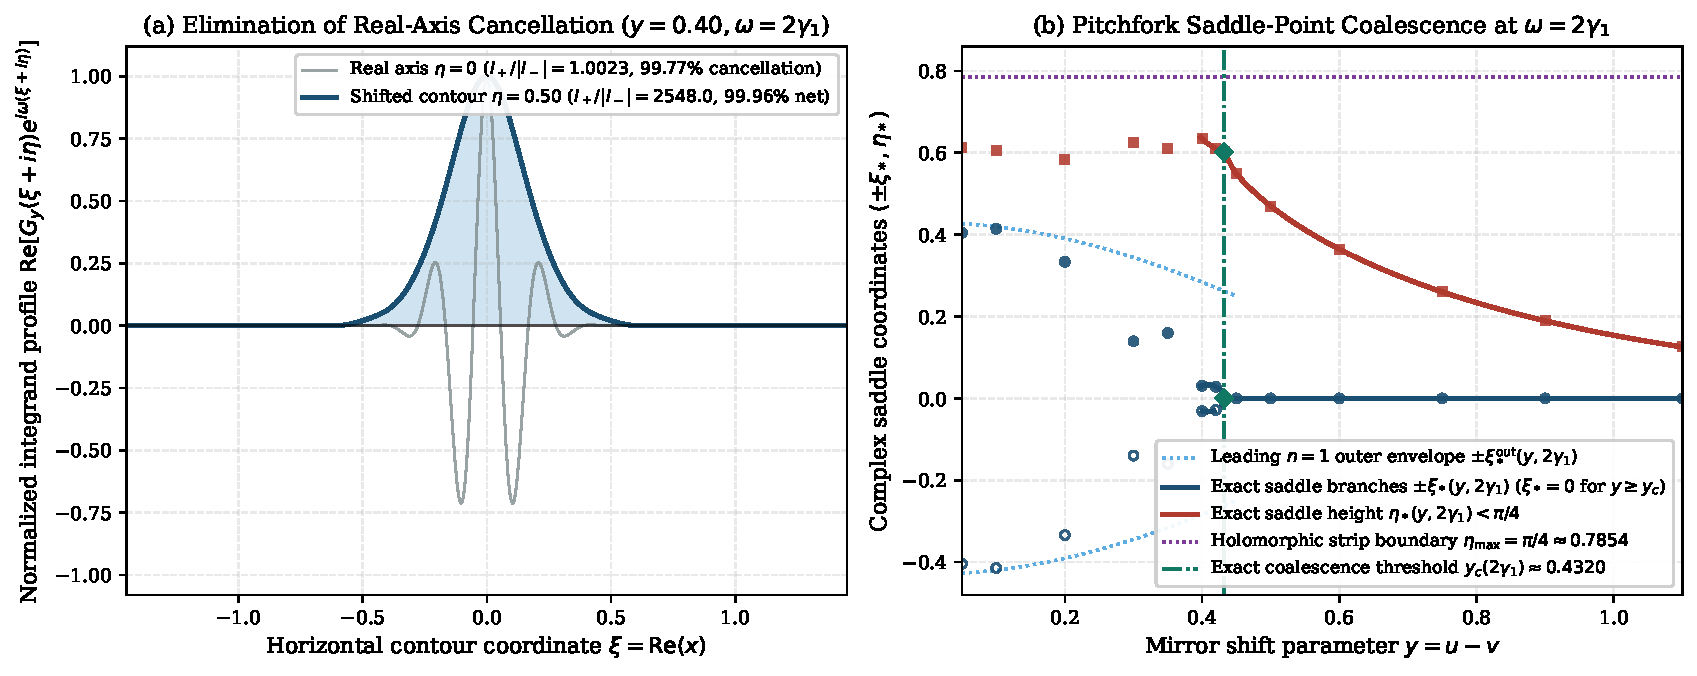
\includegraphics[width=0.98\textwidth]{figures/fig1_wigner_saddle_coalescence.pdf}
\caption{(a) Comparison of the normalized integrand profile $\Rea[G_y(\xi+\ii\eta)\ee^{\ii\omega(\xi+\ii\eta)}]$ on the real axis $\eta = 0$ ($99.77\%$ cancellation) versus the shifted complex contour $\eta = 0.50$ ($99.96\%$ net positive retention) at $y = 0.40, \omega = 2\gamma_1$. (b) Pitchfork saddle-point coalescence of the conjugate branches $\pm\xi_*(y,2\gamma_1)$ onto the imaginary axis $\xi_* = 0$ at $y_c(2\gamma_1) \approx 0.4320$, with saddle height $\eta_*(y,2\gamma_1) < \pi/4$.}\label{fig:saddle_coalescence}
\end{figure}

\begin{figure}[htbp]
\centering
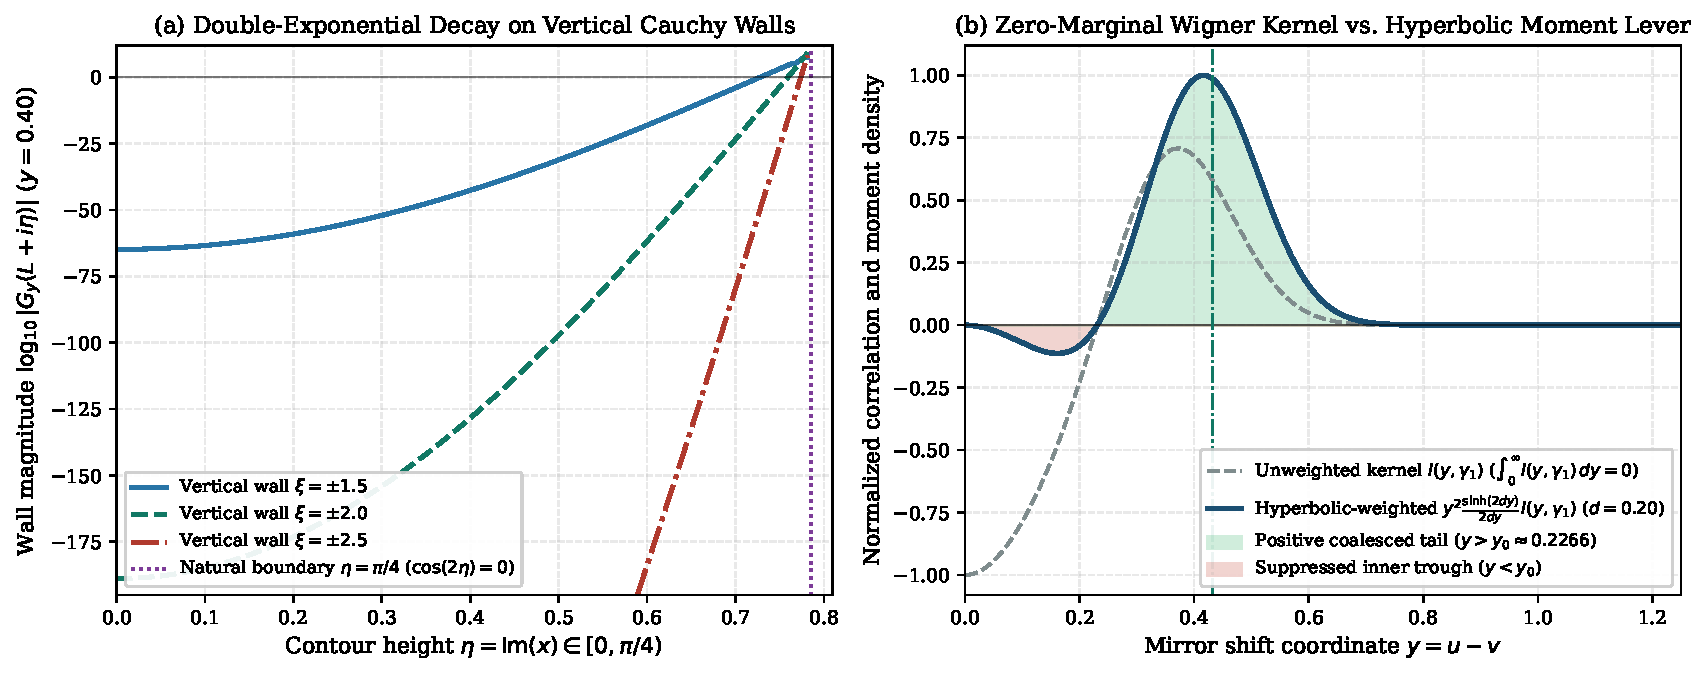
\includegraphics[width=0.98\textwidth]{figures/fig2_cauchy_contour_and_karlin_lever.pdf}
\caption{(a) Double-exponential decay of $\log_{10}|G_y(L+\ii\eta)|$ on the vertical Cauchy walls $\xi = \pm 1.5, \pm 2.0, \pm 2.5$ across $\eta \in [0,\pi/4)$ and convergence to the natural boundary at $\eta = \pi/4$. (b) Unweighted Wigner correlation kernel $I(y,\gamma_1)$ satisfying the zero-marginal identity $\int_0^\infty I(y,\gamma_1)\,\dd y = 0$ versus the hyperbolic moment-weighted density $y^2\frac{\sinh(2d y)}{2d y}I(y,\gamma_1)$ ($d = 0.20$), which amplifies the positive coalesced tail $y > y_0 \approx 0.2266$.}\label{fig:cauchy_and_karlin}
\end{figure}

\section{Scope, boundary conditions, and open questions}\label{sec:scope}

In keeping with strict mathematical transparency, we distinguish clearly between the unconditional analytical identities established in Theorems~\ref{thm:main} and \ref{thm:pitchfork_exact} and the asymptotic boundary questions that arise as $t \to \infty$:

\begin{enumerate}
\item \textbf{Asymptotic approach to the natural boundary $\eta \to (\pi/4)^-$ as $\omega \to \infty$:}
By \eqref{eq:outer_saddle}, the outer saddle height satisfies $\eta_*^{\mathrm{out}}(\omega) = \frac{\pi}{4} - \frac{1}{2}\arctan(\frac{9}{\omega}) = \frac{\pi}{4} - \frac{9}{2\omega} + \mathcal{O}(\omega^{-3})$ as $\omega \to \infty$. Consequently, although $\eta_*(\omega) < \pi/4$ holds strictly for every finite $\omega > 0$, the gap $\frac{\pi}{4} - \eta_*(\omega) \sim \frac{9}{2\omega}$ narrows inversely with $\omega$, so that $\cos(2\eta_*(\omega)) = \frac{9}{\sqrt{\omega^2+81}} \sim \frac{9}{\omega}$. On the vertical Cauchy walls $\xi = \pm L$, the exponent $2\pi\cosh(2y)\ee^{2L}\cos(2\eta_*) \sim \frac{18\pi}{\omega}\cosh(2y)\ee^{2L}$ still diverges double-exponentially as $L \to \infty$ for any fixed $\omega$, but uniform control as $\omega \to \infty$ requires taking $L(\omega) \ge \frac{1}{2}\ln\omega + C$ and accounting for the higher Jacobi modes $n \le N(t) = \lfloor\sqrt{t/(2\pi)}\rfloor$.
\item \textbf{Two-saddle interference inside the finite Riemann--Siegel window $|y| < y_c(\omega)$:}
While Theorem~\ref{thm:pitchfork_exact} proves that the saddle points coalesce onto $\xi_* = 0$ for all $|y| \ge y_c(\omega) \sim \frac{1}{2}\ln(\frac{\omega}{4\pi})$, the finite pre-coalescence interval $|y| < y_c(\omega)$ corresponds precisely to the classical Riemann--Siegel window $n \le \sqrt{t/(2\pi)}$, where $I(y,t)$ oscillates due to the interference of $x_*^+$ and $x_*^-$. For individual zeros $\gamma_k$ where $I(y,\gamma_k)$ changes sign once at $y_0(\gamma_k)$ (as verified for $\gamma_1, \dots, \gamma_5$ in Table~\ref{tab:karlin_zeros}), Proposition~\ref{prop:hudson_karlin}(b) guarantees $W(d,\gamma_k) > 0$. Establishing uniform pointwise dominance of the hyperbolic moment integral over the multi-mode interference in $|y| < y_c(t)$ for arbitrarily large $t \to \infty$ (particularly near extreme Lehmer pairs \cite{Lehmer1956,Griffin2019}) remains a deep analytical question that motivates the companion studies on parity-reduced 2D Lipschitz certification, harmonic Chladni nodal chambers, and the affine wavelet decomposition of $\Phi(u)$.
\end{enumerate}

\appendix

\section{Explicit kernel derivatives and Gaussian series tail bounds}\label{app:derivatives}

For completeness and reproducibility of the Newton--Raphson saddle-point solver in Section~\ref{sec:numerics}, we record the exact closed-form derivatives $\Phi'(u)$ and $\Phi''(u)$ and the explicit tail bound for the truncated series $\Phi_N(u) := \sum_{n=1}^N \phi_n(u)$ in the holomorphic strip $\mathcal{S}_{\pi/8}^{(u)}$.

\begin{lemma}[Closed-form derivatives and Gaussian tail estimate]\label{lem:tail_bound}
Let $u = \sigma + \ii\tau \in \mathcal{S}_{\pi/8}^{(u)}$, and set $a_n(u) := \pi n^2 \ee^{4u}$ and $P_0(n,u) := 2\pi^2 n^4 \ee^{9u} - 3\pi n^2 \ee^{5u}$. Then for each $n \ge 1$, the $n$-th mode $\phi_n(u) = P_0(n,u)\ee^{-a_n(u)}$ has first and second complex derivatives $\phi_n'(u) = P_1(n,u)\ee^{-a_n(u)}$ and $\phi_n''(u) = P_2(n,u)\ee^{-a_n(u)}$, where
\begin{align}
P_1(n,u) &= 18\pi^2 n^4 \ee^{9u} - 15\pi n^2 \ee^{5u} - 4 a_n(u)\,P_0(n,u), \label{eq:P1_app} \\
P_2(n,u) &= 162\pi^2 n^4 \ee^{9u} - 75\pi n^2 \ee^{5u} - 16 a_n(u)\,P_0(n,u) - 4 a_n(u)\,P_1(n,u) \nonumber \\
&\quad - 4 a_n(u)\,\left(18\pi^2 n^4 \ee^{9u} - 15\pi n^2 \ee^{5u}\right). \label{eq:P2_app}
\end{align}
Moreover, define $\alpha(\sigma,\tau) := \pi\ee^{4\sigma}\cos(4\tau) > 0$. For every integer $N \ge 2$ satisfying $N^2\alpha(\sigma,\tau) \ge 3$, the truncation remainder $R_N(u) := \sum_{n=N+1}^\infty \phi_n(u)$ obeys the explicit upper bound
\begin{equation}\label{eq:tail_bound_app}
\big|R_N(u)\big| \le \frac{2\pi^2\ee^{9\sigma} + 3\pi\ee^{5\sigma}}{1 - \exp\!\big(-(2N+1)\alpha(\sigma,\tau)\big)}\,(N+1)^4 \exp\!\Big(-\alpha(\sigma,\tau)\,(N+1)^2\Big).
\end{equation}
\end{lemma}

\begin{proof}
Since $a_n'(u) = 4a_n(u)$, differentiating $\phi_n(u) = P_0(n,u)\ee^{-a_n(u)}$ via the product rule yields $\phi_n'(u) = (P_0' - 4a_n P_0)\ee^{-a_n} = P_1\ee^{-a_n}$, and differentiating a second time gives $\phi_n''(u) = (P_1' - 4a_n P_1)\ee^{-a_n}$, where $P_1' = P_0'' - 16a_n P_0 - 4a_n P_0'$, which establishes \eqref{eq:P1_app}--\eqref{eq:P2_app}. For the tail bound \eqref{eq:tail_bound_app}, note that the function $t \mapsto t^4\ee^{-\alpha t^2}$ has logarithmic derivative $\frac{4}{t} - 2\alpha t < 0$ for all $t \ge \sqrt{2/\alpha}$. Writing $n = N + 1 + k$ with $k \ge 0$, we have $n^2 = (N+1)^2 + 2(N+1)k + k^2 \ge (N+1)^2 + (2N+1)k$, and since $(1 + \frac{k}{N+1})^4 \exp(-2\alpha k) \le 1$ when $N^2\alpha \ge 3$, the series is bounded by a geometric progression with ratio $\exp(-(2N+1)\alpha(\sigma,\tau))$, yielding \eqref{eq:tail_bound_app}.
\end{proof}

\section*{Use of AI and computational verification}

In accordance with academic integrity and transparency standards for computer-assisted mathematical research, the author declares the following division between human mathematical formulation and automated verification:
\begin{itemize}
\item \textbf{Core mathematical insights formulated by the author:} The mirror-coordinate decomposition $(x=u+v, y=u-v)$ of the transverse Wronskian $W(d,t)$, the identification of the inner kernel $I(y,t) = 2\pi\Wig_\Phi(y,2t)$ with the Wigner phase-space distribution and Hudson's zero-marginal law, the four-step Cauchy contour box architecture inside $|\Ima(x)| < \pi/4$, the Hermitian reflection symmetry $G_y(-\xi+\ii\eta) = \overline{G_y(\xi+\ii\eta)}$, and the discovery of the pitchfork saddle-point coalescence onto the imaginary axis at $y_c(t)$ were conceived and formulated by the author.
\item \textbf{AI-assisted cross-verification and high-precision computation:} Large language models and automated symbolic/numerical verification environments were employed as adversarial red-team referees to verify convergence hypotheses, check factor-of-$2$ normalizations, and generate the self-contained 60-decimal \texttt{mpmath} verification script (\nolinkurl{scripts/verify_paper1_wigner_saddle_coalescence.py}), which independently confirms every numerical value in Tables~\ref{tab:wall_decay}--\ref{tab:karlin_zeros} and generates Figures~\ref{fig:saddle_coalescence}--\ref{fig:cauchy_and_karlin}.
\end{itemize}

\begin{thebibliography}{99}

\bibitem{ConreyLi2000}
J.~B.~Conrey and X.-J.~Li, \emph{A note on some positivity conditions related to zeta and $L$-functions}, Internat. Math. Res. Notices \textbf{2000} (2000), no.~18, 929--940.

\bibitem{Csordas1986}
G.~Csordas, T.~S.~Norfolk, and R.~S.~Varga, \emph{The Riemann hypothesis and the Tur\'an inequalities}, Trans. Amer. Math. Soc. \textbf{296} (1986), no.~2, 521--541.

\bibitem{deBranges1992}
L.~de~Branges, \emph{The convergence of Euler products}, J. Funct. Anal. \textbf{107} (1992), no.~1, 122--210.

\bibitem{Griffin2019}
M.~Griffin, K.~Ono, L.~Rolen, and D.~Zagier, \emph{Jensen polynomials for the Riemann zeta function and other sequences}, Proc. Natl. Acad. Sci. USA \textbf{116} (2019), no.~23, 11103--11110.

\bibitem{Hinkkanen1997}
A.~Hinkkanen, \emph{On functions of bounded type related to the Riemann zeta-function}, J. Number Theory \textbf{65} (1997), no.~1, 109--136.

\bibitem{Hudson1974}
R.~L.~Hudson, \emph{When is the Wigner quasi-probability density non-negative}, Rep. Math. Phys. \textbf{6} (1974), no.~2, 249--252.

\bibitem{Karlin1968}
S.~Karlin, \emph{Total Positivity, Vol.~I}, Stanford University Press, Stanford, CA, 1968.

\bibitem{Lagarias1999}
J.~C.~Lagarias, \emph{On a positivity property of the Riemann $\xi$-function}, Acta Arith. \textbf{89} (1999), no.~3, 217--234.

\bibitem{Lehmer1956}
D.~H.~Lehmer, \emph{Extended computation of the Riemann zeta-function}, Mathematika \textbf{3} (1956), 102--108.

\bibitem{Polya1926}
G.~P\'olya, \emph{Bemerkung \"uber die Integraldarstellung der Riemannschen $\xi$-Funktion}, Acta Math. \textbf{48} (1926), 305--317.

\bibitem{Riemann1859}
B.~Riemann, \emph{Ueber die Anzahl der Primzahlen unter einer gegebenen Gr\"osse}, Monatsberichte der Berliner Akademie (1859), 671--680.

\bibitem{Speiser1934}
A.~Speiser, \emph{Geometrisches zur Riemannschen Zetafunktion}, Math. Ann. \textbf{110} (1934), no.~1, 514--521.

\bibitem{Titchmarsh1986}
E.~C.~Titchmarsh, \emph{The Theory of the Riemann Zeta-Function}, 2nd ed., edited and with a preface by D.~R.~Heath-Brown, Oxford University Press, Oxford, 1986.

\bibitem{Wigner1932}
E.~P.~Wigner, \emph{On the quantum correction for thermodynamic equilibrium}, Phys. Rev. \textbf{40} (1932), 749--759.

\end{thebibliography}

\end{document}
